\tikzset{every picture/.style={line width=0.75pt}} %set default line width to 0.75pt        

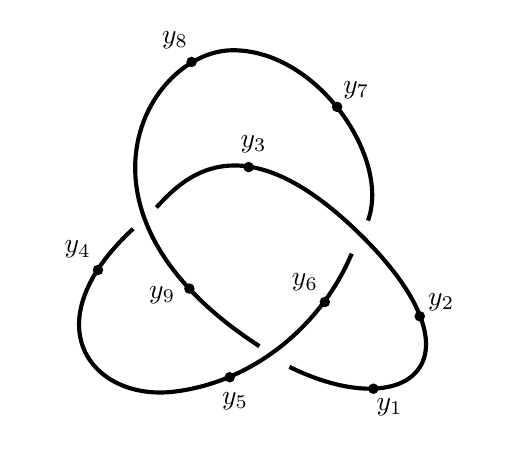
\begin{tikzpicture}[x=0.75pt,y=0.75pt,yscale=-1,xscale=1]
%uncomment if require: \path (0,300); %set diagram left start at 0, and has height of 300

%Curve Lines [id:da6513593564689459] 
\draw [color={rgb, 255:red, 0; green, 0; blue, 0 }  ,draw opacity=1 ][line width=1.5]    (390.22,157.55) .. controls (375.89,191.83) and (342.89,219.76) .. (304.07,224.11) .. controls (265.26,228.46) and (235.11,191.66) .. (284.92,145.58) ;
%Curve Lines [id:da5361254336620522] 
\draw [color={rgb, 255:red, 0; green, 0; blue, 0 }  ,draw opacity=1 ][line width=1.5]    (345.76,202.16) .. controls (246.03,137.61) and (292.04,59.77) .. (332.84,59.57) .. controls (373.64,59.36) and (409.1,111.58) .. (398.06,141.64) ;
%Curve Lines [id:da5357110084236467] 
\draw [color={rgb, 255:red, 0; green, 0; blue, 0 }  ,draw opacity=1 ][line width=1.5]    (296.11,135.3) .. controls (307.79,122.9) and (336.19,89.95) .. (396.1,150.05) .. controls (456,210.15) and (416.55,239.95) .. (360.23,212.11) ;
%Shape: Circle [id:dp4610300699755647] 
\draw  [fill={rgb, 255:red, 0; green, 0; blue, 0 }  ,fill opacity=1 ] (338.54,115.87) .. controls (338.53,114.76) and (339.42,113.86) .. (340.53,113.86) .. controls (341.63,113.85) and (342.53,114.74) .. (342.54,115.85) .. controls (342.54,116.95) and (341.65,117.85) .. (340.55,117.86) .. controls (339.44,117.86) and (338.54,116.97) .. (338.54,115.87) -- cycle ;
%Shape: Circle [id:dp7232765202765878] 
\draw  [fill={rgb, 255:red, 0; green, 0; blue, 0 }  ,fill opacity=1 ] (375.27,180.88) .. controls (375.26,179.78) and (376.15,178.88) .. (377.26,178.87) .. controls (378.36,178.87) and (379.26,179.76) .. (379.27,180.86) .. controls (379.27,181.97) and (378.38,182.87) .. (377.28,182.87) .. controls (376.17,182.88) and (375.27,181.99) .. (375.27,180.88) -- cycle ;
%Shape: Circle [id:dp5559749769028166] 
\draw  [fill={rgb, 255:red, 0; green, 0; blue, 0 }  ,fill opacity=1 ] (310.03,174.41) .. controls (310.03,173.31) and (310.92,172.41) .. (312.02,172.4) .. controls (313.13,172.4) and (314.03,173.29) .. (314.03,174.39) .. controls (314.04,175.5) and (313.15,176.4) .. (312.04,176.4) .. controls (310.94,176.41) and (310.04,175.52) .. (310.03,174.41) -- cycle ;
%Shape: Circle [id:dp682561885111596] 
\draw  [fill={rgb, 255:red, 0; green, 0; blue, 0 }  ,fill opacity=1 ] (381.19,86.85) .. controls (381.18,85.75) and (382.07,84.85) .. (383.18,84.84) .. controls (384.28,84.84) and (385.18,85.73) .. (385.19,86.83) .. controls (385.2,87.94) and (384.3,88.84) .. (383.2,88.84) .. controls (382.1,88.85) and (381.2,87.96) .. (381.19,86.85) -- cycle ;
%Shape: Circle [id:dp5688402896641405] 
\draw  [fill={rgb, 255:red, 0; green, 0; blue, 0 }  ,fill opacity=1 ] (311.08,65.21) .. controls (311.07,64.1) and (311.96,63.2) .. (313.07,63.2) .. controls (314.17,63.19) and (315.07,64.08) .. (315.08,65.19) .. controls (315.08,66.29) and (314.19,67.19) .. (313.09,67.2) .. controls (311.98,67.2) and (311.08,66.31) .. (311.08,65.21) -- cycle ;
%Shape: Circle [id:dp013108480963505365] 
\draw  [fill={rgb, 255:red, 0; green, 0; blue, 0 }  ,fill opacity=1 ] (265.99,165.44) .. controls (265.98,164.33) and (266.87,163.43) .. (267.98,163.43) .. controls (269.08,163.42) and (269.98,164.31) .. (269.99,165.42) .. controls (269.99,166.52) and (269.1,167.42) .. (268,167.43) .. controls (266.89,167.43) and (265.99,166.54) .. (265.99,165.44) -- cycle ;
%Shape: Circle [id:dp6008873411540581] 
\draw  [fill={rgb, 255:red, 0; green, 0; blue, 0 }  ,fill opacity=1 ] (329.45,217.12) .. controls (329.44,216.01) and (330.33,215.11) .. (331.44,215.11) .. controls (332.54,215.1) and (333.44,215.99) .. (333.45,217.1) .. controls (333.45,218.2) and (332.56,219.1) .. (331.46,219.11) .. controls (330.35,219.11) and (329.45,218.22) .. (329.45,217.12) -- cycle ;
%Shape: Circle [id:dp757526496728465] 
\draw  [fill={rgb, 255:red, 0; green, 0; blue, 0 }  ,fill opacity=1 ] (398.68,222.65) .. controls (398.67,221.55) and (399.56,220.65) .. (400.67,220.64) .. controls (401.77,220.64) and (402.67,221.53) .. (402.68,222.63) .. controls (402.68,223.74) and (401.79,224.64) .. (400.69,224.64) .. controls (399.58,224.65) and (398.68,223.76) .. (398.68,222.65) -- cycle ;
%Shape: Circle [id:dp013695657974363229] 
\draw  [fill={rgb, 255:red, 0; green, 0; blue, 0 }  ,fill opacity=1 ] (421.01,187.74) .. controls (421.01,186.63) and (421.9,185.73) .. (423,185.73) .. controls (424.11,185.72) and (425.01,186.61) .. (425.01,187.72) .. controls (425.02,188.82) and (424.13,189.72) .. (423.03,189.73) .. controls (421.92,189.73) and (421.02,188.84) .. (421.01,187.74) -- cycle ;

% Text Node
\draw (400.69,226.04) node [anchor=north west][inner sep=0.75pt]  [rotate=-359.71]  {$y_{1}$};
% Text Node
\draw (425.56,175.12) node [anchor=north west][inner sep=0.75pt]  [rotate=-359.71]  {$y_{2}$};
% Text Node
\draw (335.16,99.2) node [anchor=north west][inner sep=0.75pt]  [rotate=-359.71]  {$y_{3}$};
% Text Node
\draw (250.43,150) node [anchor=north west][inner sep=0.75pt]  [rotate=-359.71]  {$y_{4}$};
% Text Node
\draw (326.2,223.05) node [anchor=north west][inner sep=0.75pt]  [rotate=-359.71]  {$y_{5}$};
% Text Node
\draw (359.9,165.88) node [anchor=north west][inner sep=0.75pt]  [rotate=-359.71]  {$y_{6}$};
% Text Node
\draw (384.63,72.94) node [anchor=north west][inner sep=0.75pt]  [rotate=-359.71]  {$y_{7}$};
% Text Node
\draw (297.32,49.19) node [anchor=north west][inner sep=0.75pt]  [rotate=-359.71]  {$y_{8}$};
% Text Node
\draw (291.13,171.82) node [anchor=north west][inner sep=0.75pt]  [rotate=-359.71]  {$y_{9}$};


\end{tikzpicture}